% Options for packages loaded elsewhere
\PassOptionsToPackage{unicode}{hyperref}
\PassOptionsToPackage{hyphens}{url}
%
\documentclass[
]{book}
\usepackage{amsmath,amssymb}
\usepackage{lmodern}
\usepackage{ifxetex,ifluatex}
\ifnum 0\ifxetex 1\fi\ifluatex 1\fi=0 % if pdftex
  \usepackage[T1]{fontenc}
  \usepackage[utf8]{inputenc}
  \usepackage{textcomp} % provide euro and other symbols
\else % if luatex or xetex
  \usepackage{unicode-math}
  \defaultfontfeatures{Scale=MatchLowercase}
  \defaultfontfeatures[\rmfamily]{Ligatures=TeX,Scale=1}
\fi
% Use upquote if available, for straight quotes in verbatim environments
\IfFileExists{upquote.sty}{\usepackage{upquote}}{}
\IfFileExists{microtype.sty}{% use microtype if available
  \usepackage[]{microtype}
  \UseMicrotypeSet[protrusion]{basicmath} % disable protrusion for tt fonts
}{}
\makeatletter
\@ifundefined{KOMAClassName}{% if non-KOMA class
  \IfFileExists{parskip.sty}{%
    \usepackage{parskip}
  }{% else
    \setlength{\parindent}{0pt}
    \setlength{\parskip}{6pt plus 2pt minus 1pt}}
}{% if KOMA class
  \KOMAoptions{parskip=half}}
\makeatother
\usepackage{xcolor}
\IfFileExists{xurl.sty}{\usepackage{xurl}}{} % add URL line breaks if available
\IfFileExists{bookmark.sty}{\usepackage{bookmark}}{\usepackage{hyperref}}
\hypersetup{
  pdftitle={Supplementary Materials - CellDepot: A unified repository for scRNAseq data and visual exploration},
  hidelinks,
  pdfcreator={LaTeX via pandoc}}
\urlstyle{same} % disable monospaced font for URLs
\usepackage{color}
\usepackage{fancyvrb}
\newcommand{\VerbBar}{|}
\newcommand{\VERB}{\Verb[commandchars=\\\{\}]}
\DefineVerbatimEnvironment{Highlighting}{Verbatim}{commandchars=\\\{\}}
% Add ',fontsize=\small' for more characters per line
\usepackage{framed}
\definecolor{shadecolor}{RGB}{248,248,248}
\newenvironment{Shaded}{\begin{snugshade}}{\end{snugshade}}
\newcommand{\AlertTok}[1]{\textcolor[rgb]{0.94,0.16,0.16}{#1}}
\newcommand{\AnnotationTok}[1]{\textcolor[rgb]{0.56,0.35,0.01}{\textbf{\textit{#1}}}}
\newcommand{\AttributeTok}[1]{\textcolor[rgb]{0.77,0.63,0.00}{#1}}
\newcommand{\BaseNTok}[1]{\textcolor[rgb]{0.00,0.00,0.81}{#1}}
\newcommand{\BuiltInTok}[1]{#1}
\newcommand{\CharTok}[1]{\textcolor[rgb]{0.31,0.60,0.02}{#1}}
\newcommand{\CommentTok}[1]{\textcolor[rgb]{0.56,0.35,0.01}{\textit{#1}}}
\newcommand{\CommentVarTok}[1]{\textcolor[rgb]{0.56,0.35,0.01}{\textbf{\textit{#1}}}}
\newcommand{\ConstantTok}[1]{\textcolor[rgb]{0.00,0.00,0.00}{#1}}
\newcommand{\ControlFlowTok}[1]{\textcolor[rgb]{0.13,0.29,0.53}{\textbf{#1}}}
\newcommand{\DataTypeTok}[1]{\textcolor[rgb]{0.13,0.29,0.53}{#1}}
\newcommand{\DecValTok}[1]{\textcolor[rgb]{0.00,0.00,0.81}{#1}}
\newcommand{\DocumentationTok}[1]{\textcolor[rgb]{0.56,0.35,0.01}{\textbf{\textit{#1}}}}
\newcommand{\ErrorTok}[1]{\textcolor[rgb]{0.64,0.00,0.00}{\textbf{#1}}}
\newcommand{\ExtensionTok}[1]{#1}
\newcommand{\FloatTok}[1]{\textcolor[rgb]{0.00,0.00,0.81}{#1}}
\newcommand{\FunctionTok}[1]{\textcolor[rgb]{0.00,0.00,0.00}{#1}}
\newcommand{\ImportTok}[1]{#1}
\newcommand{\InformationTok}[1]{\textcolor[rgb]{0.56,0.35,0.01}{\textbf{\textit{#1}}}}
\newcommand{\KeywordTok}[1]{\textcolor[rgb]{0.13,0.29,0.53}{\textbf{#1}}}
\newcommand{\NormalTok}[1]{#1}
\newcommand{\OperatorTok}[1]{\textcolor[rgb]{0.81,0.36,0.00}{\textbf{#1}}}
\newcommand{\OtherTok}[1]{\textcolor[rgb]{0.56,0.35,0.01}{#1}}
\newcommand{\PreprocessorTok}[1]{\textcolor[rgb]{0.56,0.35,0.01}{\textit{#1}}}
\newcommand{\RegionMarkerTok}[1]{#1}
\newcommand{\SpecialCharTok}[1]{\textcolor[rgb]{0.00,0.00,0.00}{#1}}
\newcommand{\SpecialStringTok}[1]{\textcolor[rgb]{0.31,0.60,0.02}{#1}}
\newcommand{\StringTok}[1]{\textcolor[rgb]{0.31,0.60,0.02}{#1}}
\newcommand{\VariableTok}[1]{\textcolor[rgb]{0.00,0.00,0.00}{#1}}
\newcommand{\VerbatimStringTok}[1]{\textcolor[rgb]{0.31,0.60,0.02}{#1}}
\newcommand{\WarningTok}[1]{\textcolor[rgb]{0.56,0.35,0.01}{\textbf{\textit{#1}}}}
\usepackage{longtable,booktabs,array}
\usepackage{calc} % for calculating minipage widths
% Correct order of tables after \paragraph or \subparagraph
\usepackage{etoolbox}
\makeatletter
\patchcmd\longtable{\par}{\if@noskipsec\mbox{}\fi\par}{}{}
\makeatother
% Allow footnotes in longtable head/foot
\IfFileExists{footnotehyper.sty}{\usepackage{footnotehyper}}{\usepackage{footnote}}
\makesavenoteenv{longtable}
\usepackage{graphicx}
\makeatletter
\def\maxwidth{\ifdim\Gin@nat@width>\linewidth\linewidth\else\Gin@nat@width\fi}
\def\maxheight{\ifdim\Gin@nat@height>\textheight\textheight\else\Gin@nat@height\fi}
\makeatother
% Scale images if necessary, so that they will not overflow the page
% margins by default, and it is still possible to overwrite the defaults
% using explicit options in \includegraphics[width, height, ...]{}
\setkeys{Gin}{width=\maxwidth,height=\maxheight,keepaspectratio}
% Set default figure placement to htbp
\makeatletter
\def\fps@figure{htbp}
\makeatother
\setlength{\emergencystretch}{3em} % prevent overfull lines
\providecommand{\tightlist}{%
  \setlength{\itemsep}{0pt}\setlength{\parskip}{0pt}}
\setcounter{secnumdepth}{5}
\usepackage{booktabs}
\usepackage{amsthm}
\makeatletter
\def\thm@space@setup{%
  \thm@preskip=8pt plus 2pt minus 4pt
  \thm@postskip=\thm@preskip
}
\makeatother
\usepackage{booktabs}
\usepackage{longtable}
\usepackage{array}
\usepackage{multirow}
\usepackage{wrapfig}
\usepackage{float}
\usepackage{colortbl}
\usepackage{pdflscape}
\usepackage{tabu}
\usepackage{threeparttable}
\usepackage{threeparttablex}
\usepackage[normalem]{ulem}
\usepackage{makecell}
\usepackage{xcolor}
\ifluatex
  \usepackage{selnolig}  % disable illegal ligatures
\fi
\usepackage[]{natbib}
\bibliographystyle{apalike}

\title{Supplementary Materials - CellDepot: A unified repository for scRNAseq data and visual exploration}
\author{true \and true \and true \and true \and true \and true \and true \and true}
\date{2021-10-01}

\begin{document}
\maketitle

{
\setcounter{tocdepth}{1}
\tableofcontents
}
\hypertarget{preface}{%
\chapter{Preface}\label{preface}}

This is a CellDepot Supplementary book written in \textbf{Markdown}.

\hypertarget{getting-start-with-celldepot}{%
\chapter{Getting start with CellDepot}\label{getting-start-with-celldepot}}

\hypertarget{sources-of-annotation-and-metadata}{%
\section{Sources of annotation and metadata}\label{sources-of-annotation-and-metadata}}

The original metadata information of each single cell RNA-seq dataset is retrieved from h5ad file, which is a preferred way of sharing and storing an on-disk representation of anndata object. When importing the dataset to the system, user inputs additional metadata information as shown in Figure S5. Both metadata are collected and stored in a MySQL database table that is presented at \url{http://celldepot.bxgenomics.com}.

\hypertarget{data-format-availability-and-preparation}{%
\section{Data format, availability and preparation}\label{data-format-availability-and-preparation}}

CellDepot requires scRNA-seq data in h5ad file where the expression matrix is stored in CSC (compressed sparse column) instead of CSR (compressed sparse row) format to improve the speed of data retrieving. For example, designating genes as columns in the h5ad file creates the interactive plot five times faster than as rows. Just in case, we provide sample scripts to help users generate h5ad files. Having gene expression matrix, metadata, and layout files, users can easily combine and convert their data to h5ad file by following this R script on \url{https://github.com/interactivereport/CellDepot/blob/main/toH5ad.R}. In the case of lacking layout file, users can also create h5ad file by following the Jupyter notebook \url{https://github.com/interactivereport/CellDepot/blob/main/raw2h5ad.ipynb} with custom python script tailored to their own data. Categorical features extracted from a h5ad file are shown in the `annotation groups' column of the table on CellDepot home page, while the numerical features are shown as the distributions in the rightmost panel on cellxgene VIP

\begin{figure}
\centering
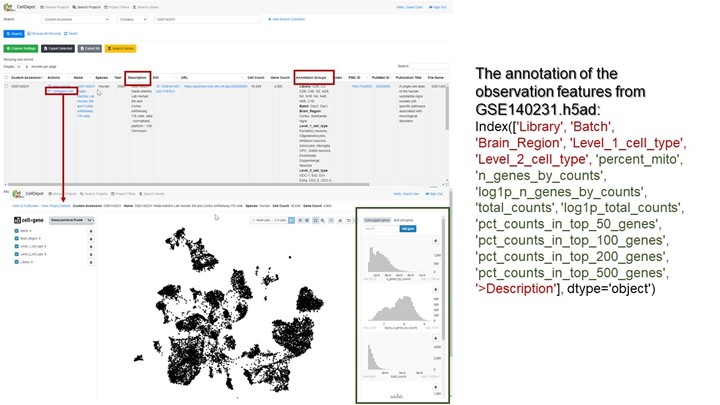
\includegraphics{figures/S3.jpg}
\caption{Figure S3. The exploration of observation features of dataset GSE140231. Red-marked categorical features are shown on CellDepot Project page (highlighted by red framed box), the numerical features marked in green color can be visualized as distribution plots on the rightmost panel in cellxgene VIP tool, which is highlighted by green box.}
\end{figure}

\hypertarget{celldepot-platform-and-installation}{%
\section{CellDepot platform and installation}\label{celldepot-platform-and-installation}}

The public version of CellDepot web portal is hosted at the web site, \url{http://celldepot.bxgenomics.com} and is implemented with MySQL database, an advanced search engine, and powerful interactive visualizing tools that allow users to explore attributes of datasets as well as scRNA-seq analysis results. Also, users can intentionally select single-cell RNA-seq datasets on the web interface by simply browsing the online dataset table or applying advanced search to perform the cross-dataset comparison. Moreover, CellDepot also provides comprehensive data analysis tools via an embedded interactive visualization plugin. To host private datasets, local instance of CellDepot on Unix server can be installed by following the guide here, \url{https://celldepot.bxgenomics.com/celldepot_manual/install_environment.php}.

\hypertarget{data-import-on-users-server}{%
\section{Data import on user's server}\label{data-import-on-users-server}}

The prepared h5ad files are required to copy to a folder defined in the configuration file, e.g., /data/celldepot/all\_h5ad\_files/. Afterwards, users can navigate to the CellDepot home page, click `Import Project' at the top menu, then `Download Example File' to fill in meta information of datasets into the downloaded template for submission. After the metadata file is uploaded, CellDepot will automatically convert the dataset to CSC format if needed through a cron job (Supplementary Tutorial Section 5). To explore the detail of imported datasets, users can enter `Browse Projects' page and then search these datasets by user assigned accessions in the metadata file.

\hypertarget{celldepot-api-application-programming-interface}{%
\section{CellDepot API (Application Programming Interface)}\label{celldepot-api-application-programming-interface}}

The CellDepot API web service provides a direct way to generate figures for users to share or embed in web page. For example, the following URL will generate a gene expression violin plot across cell clusters for IRAK4 gene for the data set with ID equaling one, \url{https://celldepot.bxgenomics.com/celldepot/app/core/api_gene_plot.php?ID=1\&Genes=IRAK4\&Plot_Type=violin\&Subsampling=0\&n=0\&g=0\&Project_Group=CLUSTER}. The complete format of the URL and explanation of parameters are detailed in the web page, \url{https://celldepot.bxgenomics.com/celldepot_manual/api_gene_plot.php}.

\hypertarget{code-availability}{%
\section{Code availability}\label{code-availability}}

The source code, local installation guide and complete tutorial of visualization and analysis tool are provided at \url{https://github.com/interactivereport/CellDepot}. With broad adoption and contribution in mind, CellDepot is released under the MIT License.

\hypertarget{SITable}{%
\chapter{Supplementary Tables}\label{SITable}}

\hypertarget{comparsion-matrix-of-web-portal-tools}{%
\section{Comparsion matrix of web portal tools}\label{comparsion-matrix-of-web-portal-tools}}

\begin{table}

\caption{\label{tab:unnamed-chunk-2}Comparsion matrix of web portal tools}
\centering
\begin{tabular}[t]{l|l|l|l|l|l|l|l|l|l|l|l|l|l|l}
\hline
Web.application.repository & CellDepot & Corpora.Data.Portal & gEAR & CHARTS & SCANNER & Single.Cell.Portal & ReproGenomics & PanglaoDB & Expression.Atlas & scRNAseqDB & conquer & JingleBells & Human.Cell.ATLAS & Sfaira\\
\hline
Year & 2021 & 2021 & 2021 & 2020 & 2020 & 2020 & 2019 & 2019 & 2019 & 2019 & 2018 & 2017 & 2017 & 2020\\
\hline
Main Function &  &  &  &  &  &  &  &  &  &  &  &  &  & \\
\hline
Database Explorer & Y & Y & Y & Y & NA & Y & Y & Y & Y & Y & Y & Y & Y & Y\\
\hline
Query Search & Advanced & NA & Basic I & NA & Intermediate & Advanced & Intermediate & Advanced & Intermediate & Basic I & Basic I & Basic I & Advanced & Basic II\\
\hline
Data Analysis Explorer & Advanced & Advanced & Advanced & Intermediate & Intermediate & Intermediate - Advanced & Basic & Intermediate & Intermediate & Basic - Intermediate & Basic & NA & NA & NA\\
\hline
Data Type supported &  &  &  &  &  &  &  &  &  &  &  &  &  & \\
\hline
Datasets & divserse & divserse & hearing/brain & tumor & diverse & diverse & reproduction & diverse & diverse & diverse & diverse & immune-related & diverse & diverse\\
\hline
Datatypes & Single-cell & Single-cell & Single-cell, Epigenetics & Single-cell & Single-cell & Single-cell & Single-cell, Multi-omics & Single-cell & Single-cell, Protemics & Single-cell & Single-cell & Single-cell & Single-cell, Multi-omics & Single-cell\\
\hline
Visualzation features & Violin, dot, heatmap, bar, QC, scatter, density, embed-ding plots & Bar, scatter, embeddeing plots & Violin, dot, line, bar, QC, embed-ding plots, genome browser & Bar, embed-ding plots & Violin, dot, scatter, & Violin, scatter, heatmap, embedding plots & Violin, density, scatter plots, genome browser & Bar, QC, scatter, embedding plots & Heatmap, scatter. embedding plots & Scatter, bar plots & Scatter, QC plots & Genome browser & NA & NA\\
\hline
Links &  &  &  &  &  &  &  &  &  &  &  &  &  & \\
\hline
Source Code link & https://github.com/interactivereport/CellDepot & https://github.com/chanzuckerberg/single-cell-data-portal & https://github.com/IGS/gEAR & https://github.com/stewart-lab/CHARTS & https://github.com/GuoshuaiCai/scanner & https://github.com/broadinstitute/single\_cell\_portal\_core & https://github.com/fchalmel/RGV & https://github.com/oscar-franzen/PanglaoDB & https://github.com/ebi-gene-expression-group/atlas & NA & https://github.com/csoneson/conquer\_comparison & https://drive.google.com/drive/folders/0BxSFjdiDhUI1amNoSks0SmpMdE0?resourcekey=0-s7Qw02gR8VhkS7hfdE9nPg & https://github.com/HumanCellAtlas/ & https://github.com/theislab/sfaira-portal\\
\hline
Demo link & http://celldepot.bxgenomics.com/ & https://cellxgene.cziscience.com/ & umgear.org & https://charts.morgridge.org & https://www.thecailab.com/scanner/ & https://singlecell.broadinstitute.org/single\_cell & https://rgv.genouest.org/ & https://panglaodb.se & https://www.ebi.ac.uk/gxa/sc/home & https://bioinfo.uth.edu/scrnaseqdb/ & http://imlspenticton.uzh.ch:3838/conquer/ & https://jinglebells.bgu.ac.il/ & https://data.humancellatlas.org/ & https://theislab.github.io/sfaira-portal/About\\
\hline
\end{tabular}
\end{table}

Note: The criteria for query search and data analysis explorer please see Table S2 and S3.

\hypertarget{criterion-for-query-search}{%
\section{Criterion for query search}\label{criterion-for-query-search}}

\begin{table}

\caption{\label{tab:unnamed-chunk-3}Criterion for query searchs}
\centering
\begin{tabular}[t]{l|l|l|l}
\hline
Query.Search & Keyword.Search & Multiple.Object.Search & Category.Filters\\
\hline
Basic S2 & Y &  & \\
\hline
Basic II &  &  & Y\\
\hline
Intermediate & Y &  & Y\\
\hline
Advanced & Y & Y & Y\\
\hline
\end{tabular}
\end{table}

\hypertarget{criterion-for-data-analysis-explorer}{%
\section{Criterion for data analysis explorer}\label{criterion-for-data-analysis-explorer}}

\begin{table}

\caption{\label{tab:unnamed-chunk-4}Criterion for data analysis explorer}
\centering
\begin{tabular}[t]{l|l|l|l}
\hline
Data.Analysis.Explorer & Analyze.scRNAseq.Data & Anaylze.Gene.Expression & Customize.Displays\\
\hline
Basic & Y &  & \\
\hline
Intermediate & Y & Y & \\
\hline
Advanced & Y & Y & Y\\
\hline
\end{tabular}
\end{table}

\hypertarget{project-metadata-captured-in-celldepot}{%
\section{Project metadata captured in CellDepot}\label{project-metadata-captured-in-celldepot}}

\begin{table}

\caption{\label{tab:unnamed-chunk-5}Project metadata captured in CellDepot}
\centering
\begin{tabular}[t]{l|l|l|l}
\hline
X & General.Category & Expected.Variable.Type & Description\\
\hline
Project Browser/Search &  &  & \\
\hline
 & Annotation Groups & String & categorical  features from h5ad file\\
\hline
 & Cell Count & Integer & numbers of cell in study\\
\hline
 & Actions & Link & three options: 1) Study summary information; 2) Data visualization and analysis; 3) Update project information\\
\hline
 & Custom Accession & String & Customized accession name for individual project\\
\hline
 & Description & String & Additional information\\
\hline
 & DOI & Link & Digtial Object Identifier\\
\hline
 & File Name & String & h5ad file name\\
\hline
 & File Size & Integer & size of h5ad file\\
\hline
 & Gene Count & Integer & numbers of gene in study\\
\hline
 & Name & Link & project name\\
\hline
 & Notes & String & study notes\\
\hline
 & PMC ID & Link & \\
\hline
 & Publication Title &  & \\
\hline
 & PubMed ID & Link & \\
\hline
 & Speices & String & \\
\hline
 & URL & Link & \\
\hline
 & Year & String & \\
\hline
\end{tabular}
\end{table}

\hypertarget{SITutorial}{%
\chapter{Supplementary Tutorial}\label{SITutorial}}

CellDepot is database management system integrated with management system, query searching and data visualization tools {[}2, 3{]} for scRNA-seq datasets, which can be accessed by the link \url{http://celldepot.bxgenomics.com}. This is a supplemental tutorial provides a detailed guide.

\begin{figure}
\centering
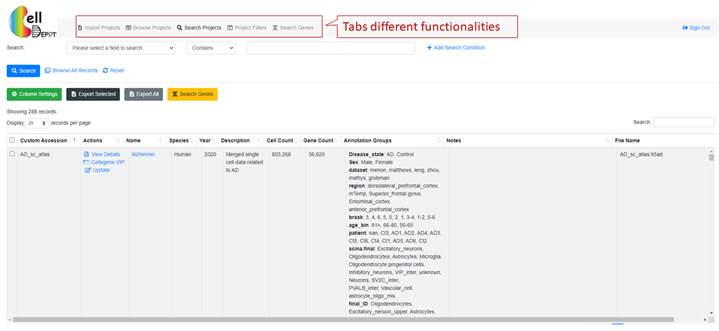
\includegraphics{figures/S4.png}
\caption{Figure S1. CellDepot website}
\end{figure}

The interface contains multiple tabs, corresponding to import and/or select objects in CellDepot scRNA-seq database, that can be accessed on top panel of the webpage. Users can upload their own dataset or explore the existing datasets for visualization and analysis.

\hypertarget{upload-projects}{%
\section{Upload Projects}\label{upload-projects}}

To upload new projects in CellDepot database, two files are required: 1) .h5ad files and 2) project information in csv format. Detailed formatting guidance can be found by `Download Example File' hyperlink on webpage. In addition, two cellxgene VIP launch methods are provided: standard and preload in memory. Standard mode is for the first-time imported datasets, while preload in memory should be chosen when users update the meta information of datasets.
After the projects are submitted, CellDepot will automatically analyze the datasets. To explore the detail of uploaded datasets, users can navigate to `browse projects' page and then search the imported datasets by the customized accession number.

\begin{figure}
\centering
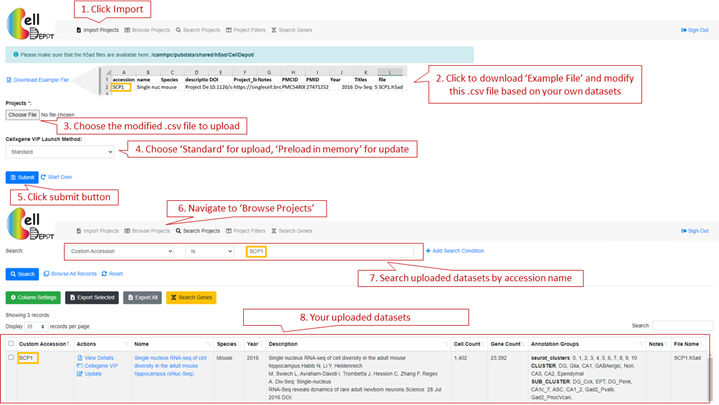
\includegraphics{figures/S5.png}
\caption{Figure S5. Workflow of how to import personal datasets.}
\end{figure}

\hypertarget{browse-projects}{%
\section{Browse Projects}\label{browse-projects}}

\hypertarget{search-projects}{%
\subsection{Search Projects}\label{search-projects}}

This function allows the user to search any targeted interests, which also can be accessed through search projects on the top panel of the webpage. Users is allowed to select the projects by 17 attributes: annotation groups, cell count, cellxgene VIP launch method, Custom accession, description, DOI, file name, file size, gene count, name, notes, PMC ID, Publication Title, PubMed ID, Species, URL, Year. These 17 fields can also be (partially) displayed on the webpage through `column setting' on the webpage. Users can also search projects by the keywords via the search function on the right of the webpage. In addition, by `column setting', users can set up the customized layout of targeted projects; thereby exporting to csv format.

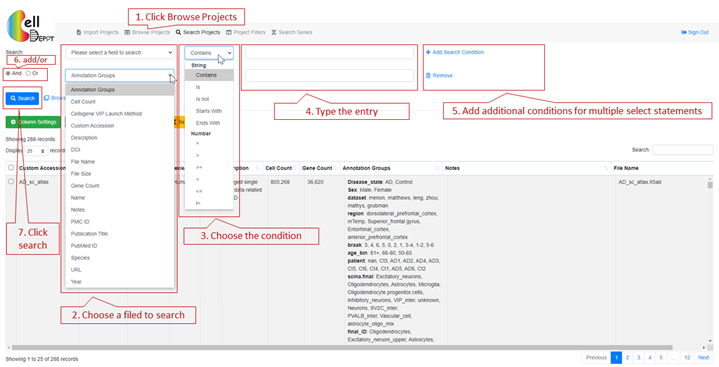
\includegraphics{figures/S6.png}
\#\#\#\# Case study 1

Six datasets are filtered when searching by `Species is Human' and `Annotation Group contains Neuron'.

\begin{figure}
\centering
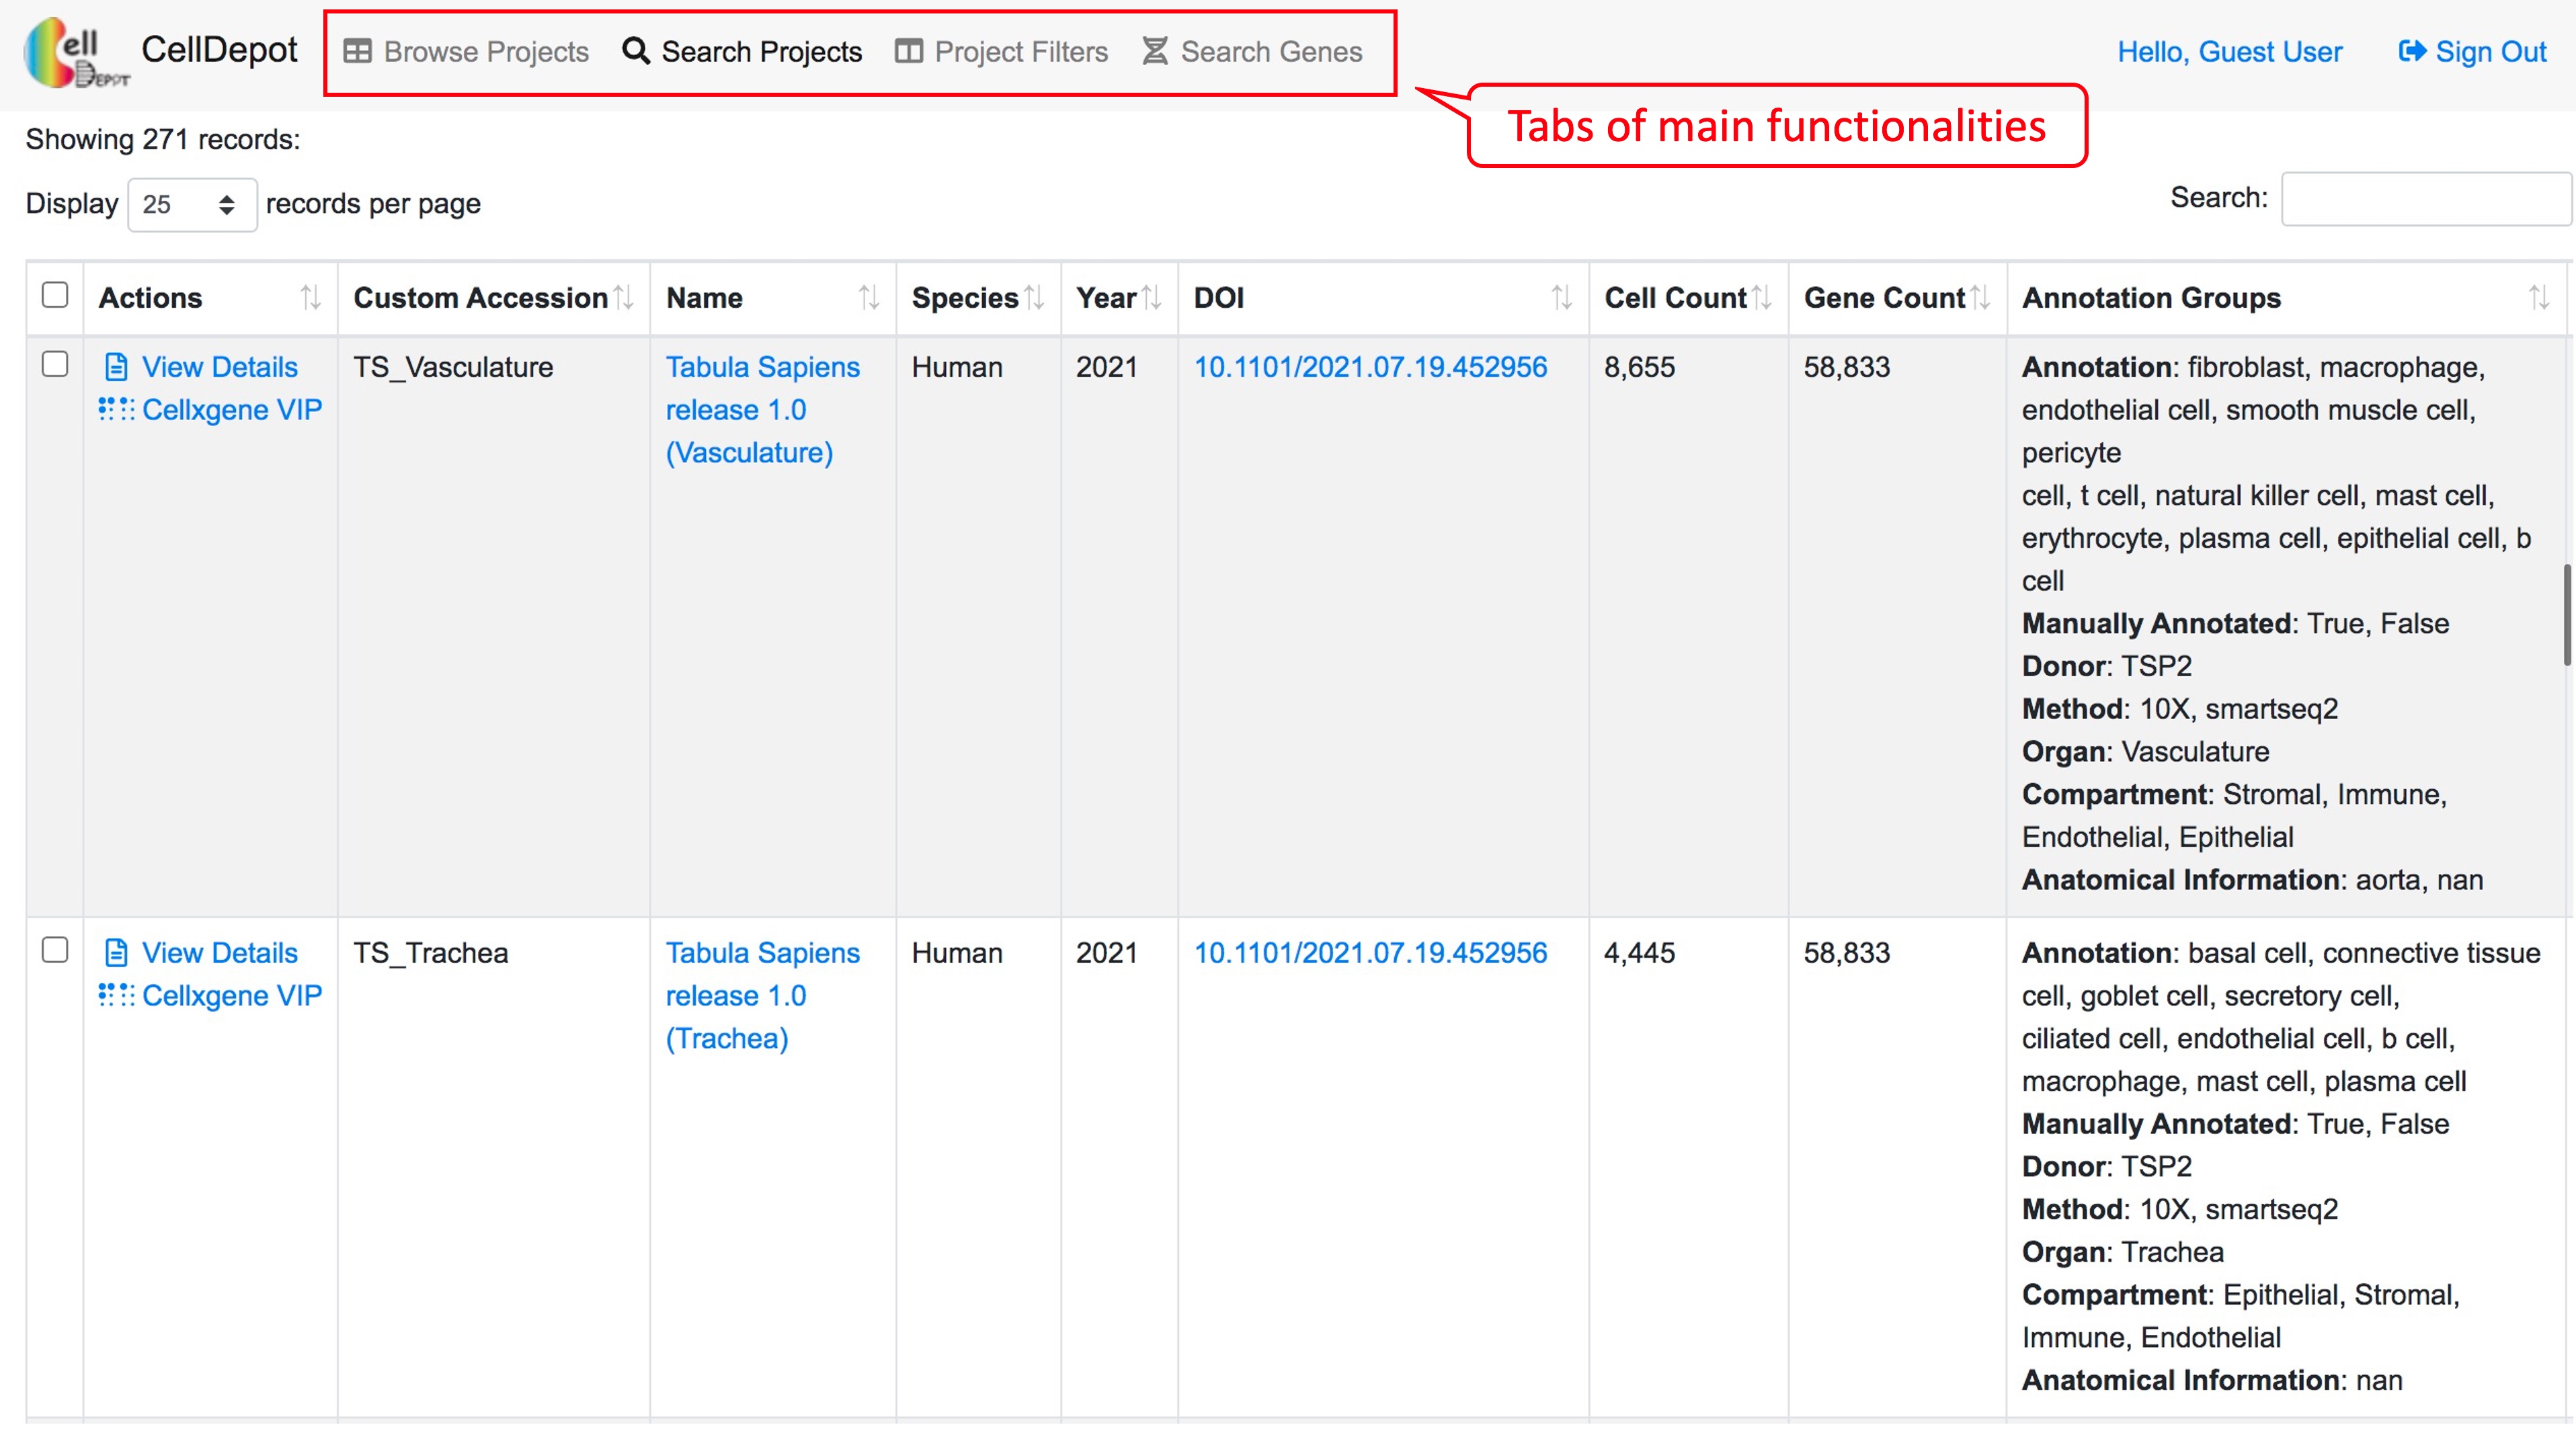
\includegraphics{figures/S1.jpg}
\caption{Figure S1. Data Filtering. Query search of `Species is Human' and `Annotation Groups contains Neuron' brings about nine datasets of interest.}
\end{figure}

\hypertarget{case-study-2}{%
\subsubsection{Case Study 2}\label{case-study-2}}

Cross-project comparison of skeletal muscle marker genes PAX3, PAX7, PITX2, MYF5, MYF6, MYOD1, MYOG, NEB, and MYH3 among the datasets whose species is human and cell type is myogenic.

\begin{figure}
\centering
\includegraphics{figures/s7.png}
\caption{Figure S7. Workflow of how to conduct the cross-project comparison of gene sets among the selected datasets.}
\end{figure}

For each project, users can view the datasets information, visualize data analysis, and conduct update through clicking on ``View Details'', ``cellxgene VIP'', and ``Update'' links, respectively.

\hypertarget{project-filters}{%
\subsection{Project Filters}\label{project-filters}}

This page provides the matched datasets by simply clicking the categories. It is a first-time user-friendly functionality as users may not be familiar with the content of the database. The advance search function is the same as that on the `Browse Projects' page (Details see Figure S4).

\begin{figure}
\centering
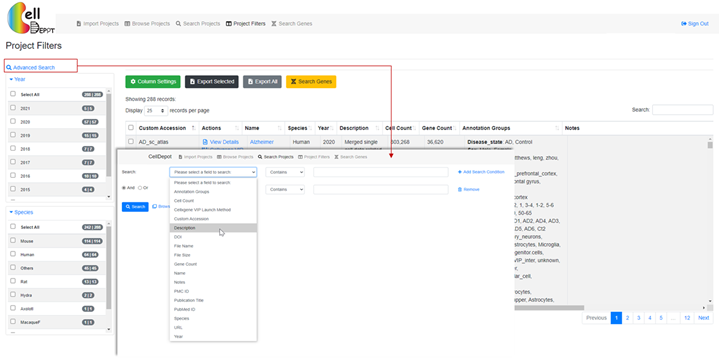
\includegraphics{figures/S8.png}
\caption{Figure S8. The layout of `Project Filters' page.}
\end{figure}

\hypertarget{visaulize-datasets}{%
\section{Visaulize Datasets}\label{visaulize-datasets}}

\hypertarget{view-details}{%
\subsection{View Details}\label{view-details}}

The datasets information consists of project summary and annotation groups. The project summary is provided by each user when uploading projects. The information of annotation groups is retrieved from uploaded .h5ad file.

\begin{figure}
\centering
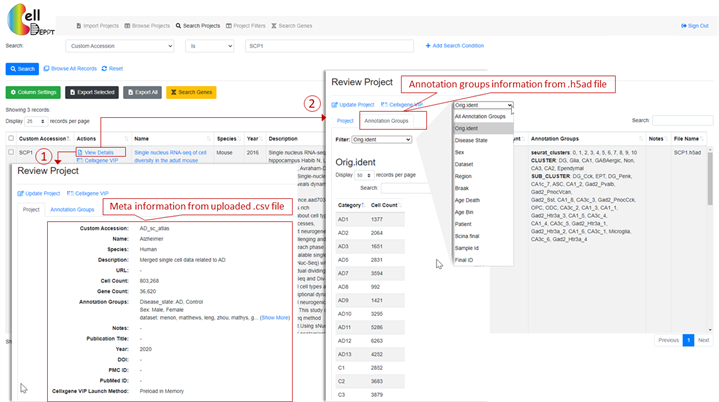
\includegraphics{figures/S9.png}
\caption{Figure S9. Visualization of details of datasets.}
\end{figure}

\hypertarget{update}{%
\subsection{Update}\label{update}}

Project summary information can be updated on `Browse Project' page with `Preload in Memory' cellxgene VIP launch method via click `Update' hyperlink.

\begin{figure}
\centering
\includegraphics{figures/s10.png}
\caption{Figure S10. Update project on `Browse Project' page.}
\end{figure}

\hypertarget{data-visualization-and-analysis}{%
\subsection{Data Visualization and Analysis}\label{data-visualization-and-analysis}}

CellDepot is not only a database management system, but also a web portal to visualize the scRNA-seq dataset. Here, we embed cellxgene and cellxgene VIP in CellDepot. By clicking `Cellxgene VIP', data analysis results can be visualized. Detailed guides of cellxgene and cellxgene VIP, please go to \url{https://interactivereport.github.io/cellxgene_VIP/tutorial/docs/}.

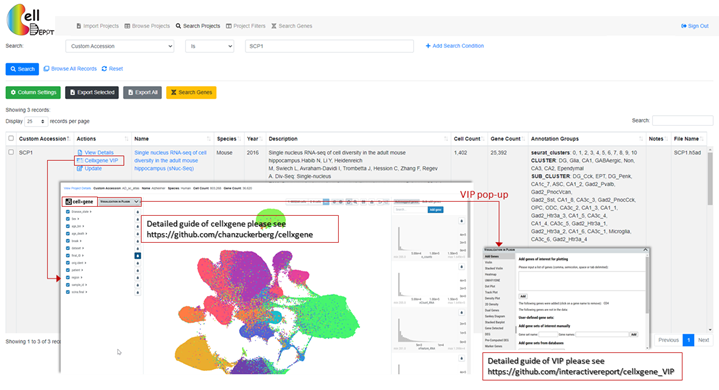
\includegraphics{figures/S11.png}
\#\#\#\# Case study 1
Exploration and visualization of the expression of gene(s) across the cluster of cells under various conditions.As shown in Figure S2a, two cell groups from Astrocytes (1036 cells) and Oligodendrocytes (4417 cells) are selected. By running differential analysis with one of the built-in statistical methods such as Welch's t-test, we detected 1578 differential expressed genes (DEGs), including 715 up-regulated and 853 down-regulated genes in astrocytes compared to oligodendrocytes (Figure S2a). The expression of the top four DEGs among the cell types indicates that gene MBP, ST18 and RNF220 are expressed explicitly in oligodendrocytes, while gene PITPNC3 is expressed mainly in astrocytes and endothelial cells (Figure S2b). In the future, we plan to add other multi-omics data modalities, which can be incorporated and integrated with scRNA-seq, such as spatial transcriptomics and scATAC-seq data.
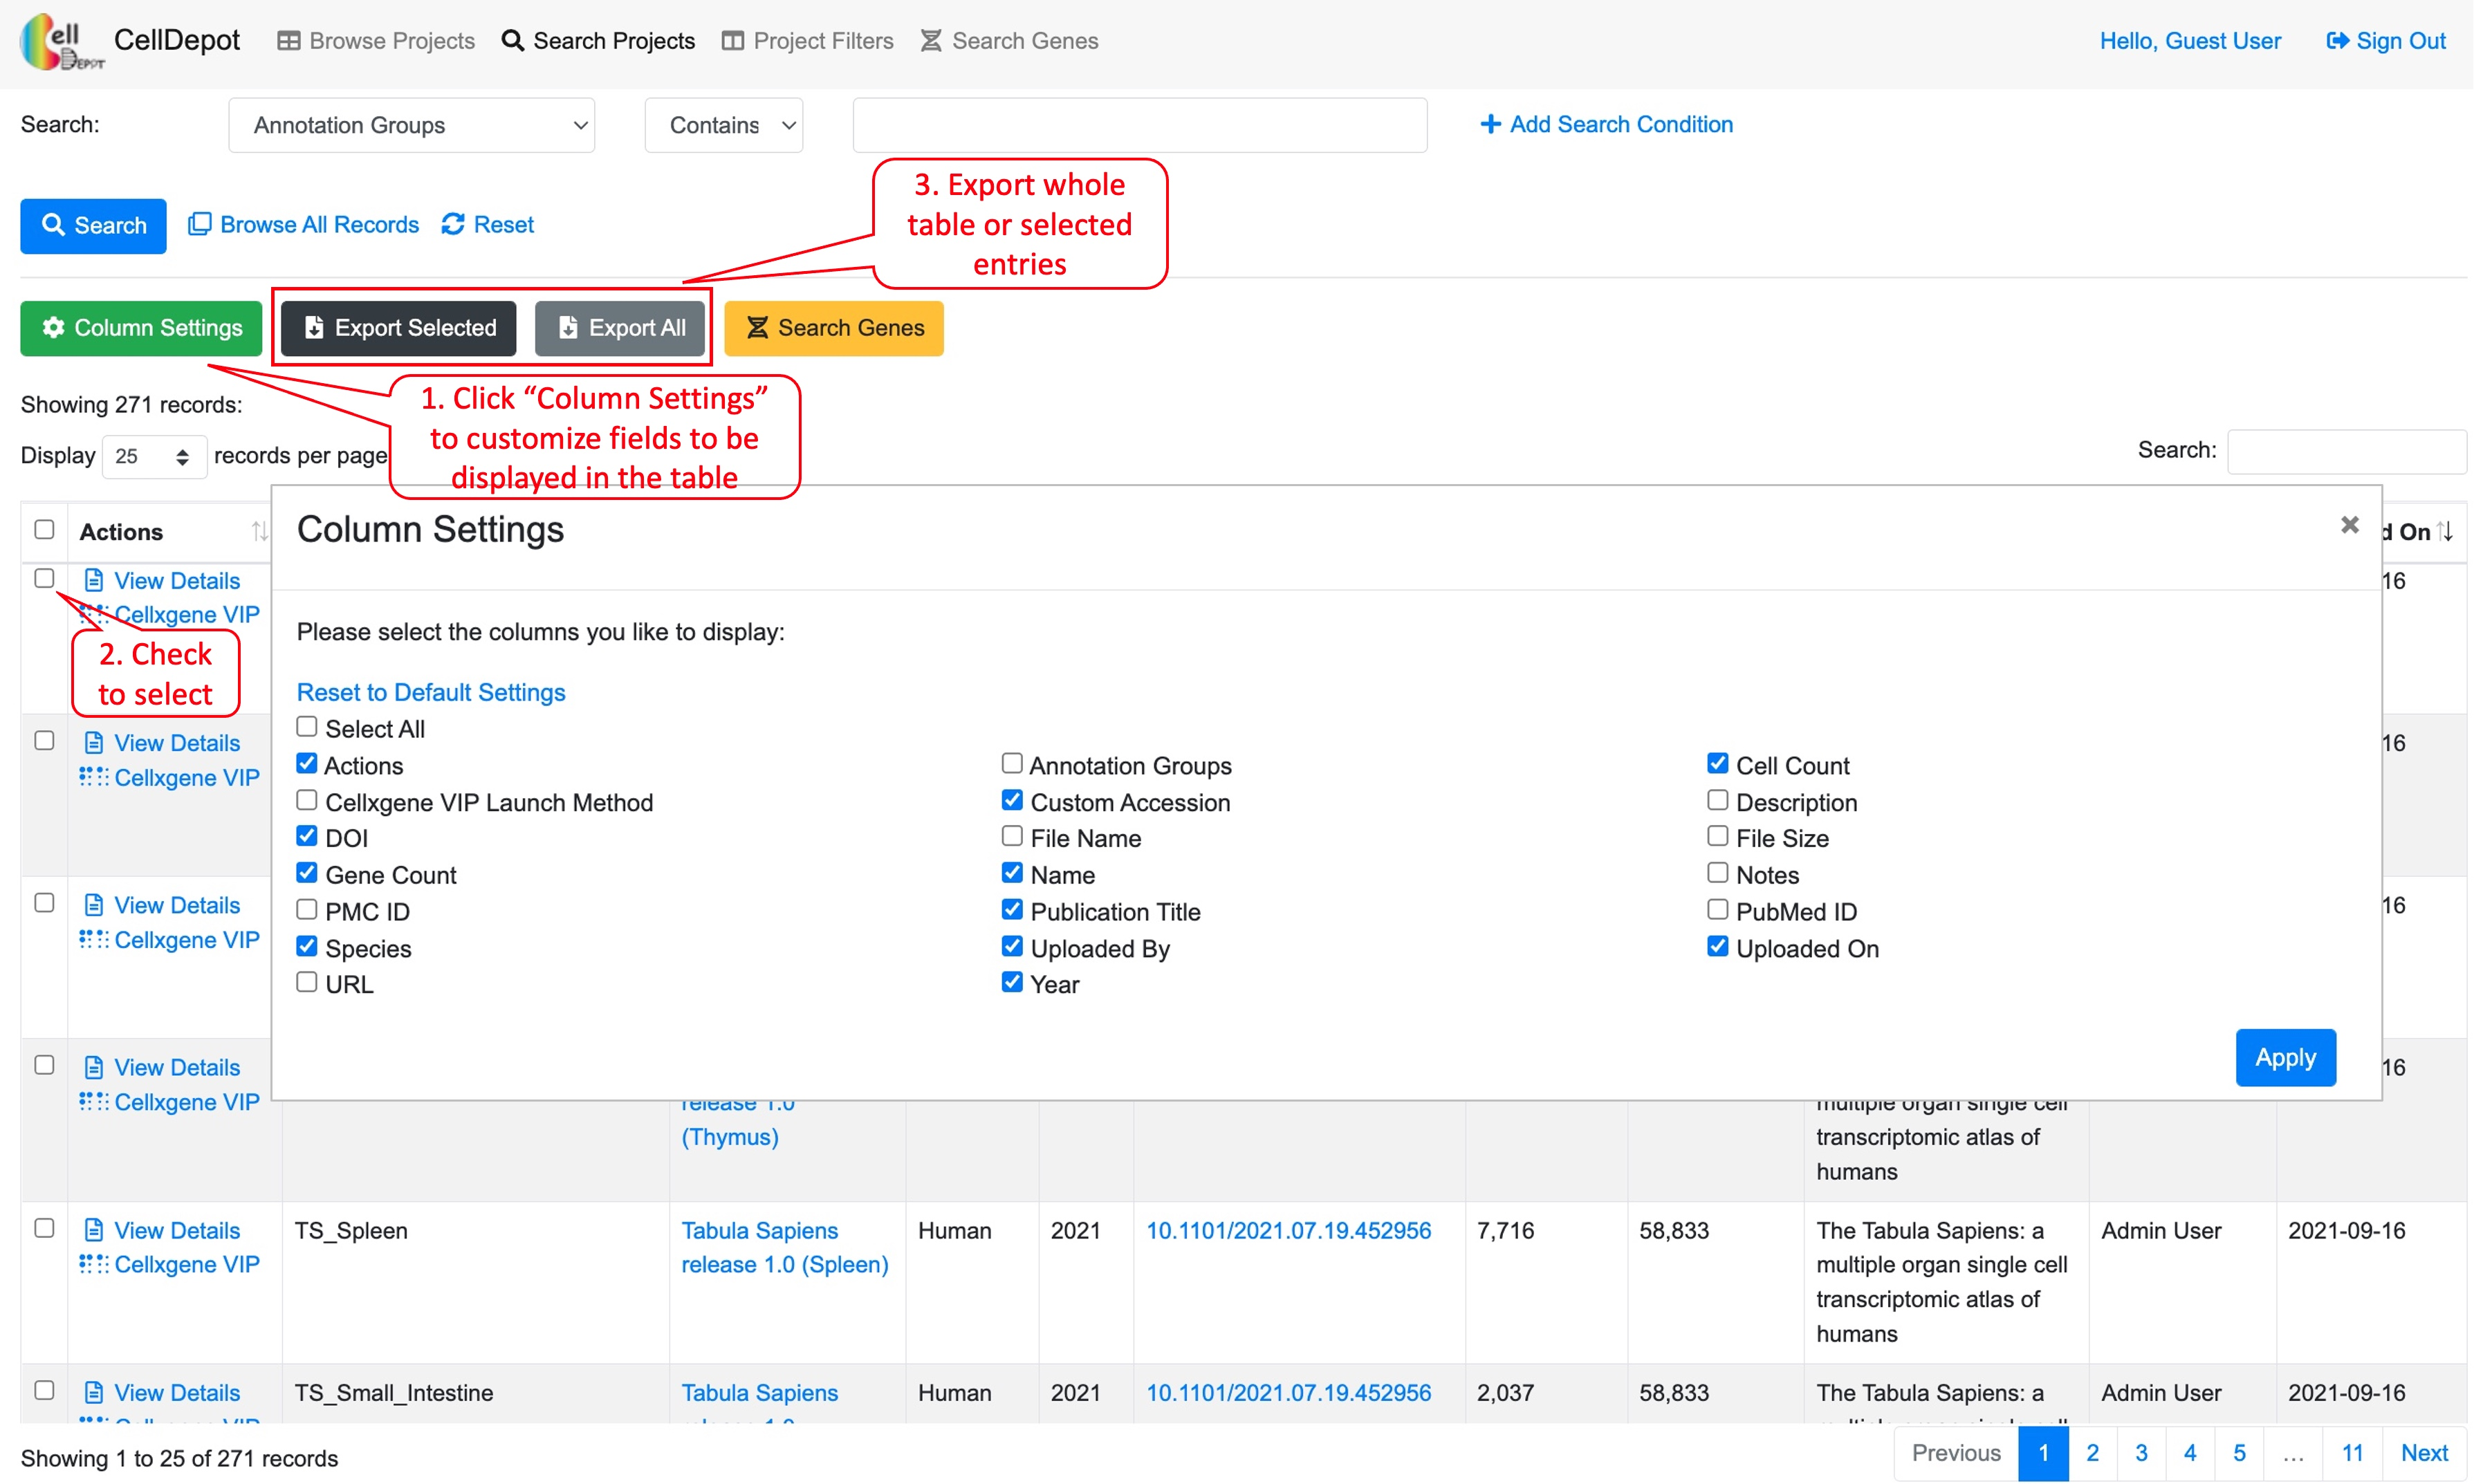
\includegraphics{figures/S2.jpg}

\hypertarget{search-genes}{%
\section{Search Genes}\label{search-genes}}

This tab allows searching on targeted genes with cell count cutoff and expression cutoff. The search outcome provides users every project contains the targeted genes. Each project displays a link to project page and a figure plot if applicable. This plot can be either violin plot or dot plot shows the gene expression level in each annotation groups.

\begin{figure}
\centering
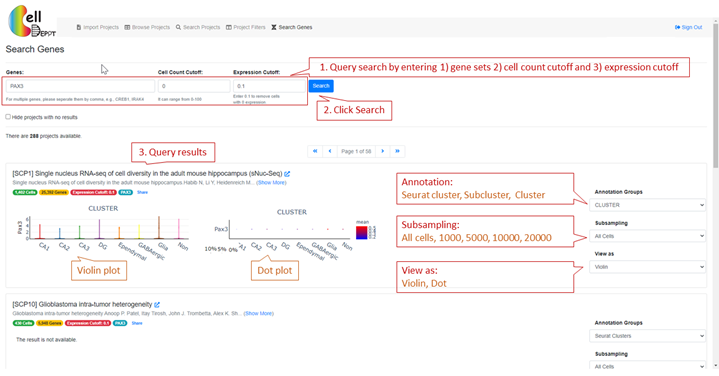
\includegraphics{figures/S12.png}
\caption{Figure S12. The layout of `Search Genes'}
\end{figure}

\hypertarget{how-to-set-up-cron-job}{%
\section{How to set up cron job?}\label{how-to-set-up-cron-job}}

The following cron job entry is needed to convert h5ad file to CSC format on the background,

\begin{Shaded}
\begin{Highlighting}[]
\ExtensionTok{@hourly} \OperatorTok{\textless{}}\NormalTok{user{-}name}\OperatorTok{\textgreater{}}\NormalTok{ cd /var/www/html/celldepot/app/core}\KeywordTok{;} \ExtensionTok{php}\NormalTok{ ./api\_toCSCh5ad.php}
\end{Highlighting}
\end{Shaded}

Please make sure that the user has the permission to write in the data directory.

  \bibliography{book.bib,packages.bib}

\end{document}
